\documentclass[sigconf,table,9pt]{acmart}

\usepackage{algpseudocode}
\usepackage{algorithm}
\usepackage{algorithmicx}
\usepackage{verbatim}
\usepackage{mathtools}
\usepackage{multirow}
\usepackage{subcaption}
\usepackage{colortbl}
\usepackage{balance}
\usepackage{extarrows}

\usepackage{tikz}
\usetikzlibrary{automata,positioning}

\definecolor{lightgray}{gray}{0.9}


%\def\BibTeX{{\rm B\kern-.05em{\sc i\kern-.025em b}\kern-.08em
%	T\kern-.1667em\lower.7ex\hbox{E}\kern-.125emX}}

\usepackage{booktabs} % For formal tables


\newlength\Origarrayrulewidth

% horizontal rule equivalent to \cline but with 2pt width
\newcommand{\Cline}[1]{%
	\noalign{\global\setlength\Origarrayrulewidth{\arrayrulewidth}}%
	\noalign{\global\setlength\arrayrulewidth{3pt}}\cline{#1}%
	\noalign{\global\setlength\arrayrulewidth{\Origarrayrulewidth}}%
}

% draw a vertical rule of width 2pt on both sides of a cell
\newcommand\Thickvrule[1]{%
	\multicolumn{1}{!{\vrule width 2pt}c!{\vrule width 2pt}}{#1}%
}

% draw a vertical rule of width 2pt on the left side of a cell
\newcommand\Thickvrulel[1]{%
	\multicolumn{1}{!{\vrule width 2pt}c}{#1}%
}

% draw a vertical rule of width 2pt on the right side of a cell
\newcommand\Thickvruler[1]{%
	\multicolumn{1}{c!{\vrule width 2pt}}{#1}%
}

%%
%% \BibTeX command to typeset BibTeX logo in the docs
\AtBeginDocument{%
	\providecommand\BibTeX{{%
			\normalfont B\kern-0.5em{\scshape i\kern-0.25em b}\kern-0.8em\TeX}}}

%% Rights management information.  This information is sent to you
%% when you complete the rights form.  These commands have SAMPLE
%% values in them; it is your responsibility as an author to replace
%% the commands and values with those provided to you when you
%% complete the rights form.

\copyrightyear{2021}
\acmYear{2021}
\setcopyright{acmlicensed}\acmConference[GRADES-NDA'21]{4th Joint International Workshop on Graph Data Management Experiences \& Systems (GRADES) and Network Data Analytics (NDA)}{June 20--25, 2021}{Virtual Event, China}
\acmBooktitle{4th Joint International Workshop on Graph Data Management Experiences \& Systems (GRADES) and Network Data Analytics (NDA) (GRADES-NDA'21), June 20--25, 2021, Virtual Event, China}
\acmPrice{15.00}
\acmDOI{10.1145/3461837.3464513}
\acmISBN{978-1-4503-8477-3/21/06}


%%
%% Submission ID.
%% Use this when submitting an article to a sponsored event. You'll
%% receive a unique submission ID from the organizers
%% of the event, and this ID should be used as the parameter to this command.
%%\acmSubmissionID{123-A56-BU3}

%%
%% The majority of ACM publications use numbered citations and
%% references.  The command \citestyle{authoryear} switches to the
%% "author year" style.
%%
%% If you are preparing content for an event
%% sponsored by ACM SIGGRAPH, you must use the "author year" style of
%% citations and references.
%% Uncommenting
%% the next command will enable that style.
%%\citestyle{acmauthoryear}

\newtheorem{mytheorem}{Theorem}
\newtheorem{myproposition}{Proposition}

\newcommand{\ltz}{$< 1$}

\algtext*{EndWhile}% Remove "end while" text
\algtext*{EndIf}% Remove "end if" text
\algtext*{EndFor}% Remove "end for" text
\algtext*{EndFunction}% Remove "end function" text

%%
%% end of the preamble, start of the body of the document source.
\begin{document}
	\fancyhead{}
	
	%%
	%% The "title" command has an optional parameter,
	%% allowing the author to define a "short title" to be used in page headers.
	\title[]{Context-Free Path Querying with All-Path Semantics by Matrix Multiplication}
	
	%%
	%% The "author" command and its associated commands are used to define
	%% the authors and their affiliations.
	%% Of note is the shared affiliation of the first two authors, and the
	%% "authornote" and "authornotemark" commands
	%% used to denote shared contribution to the research.
	
	
	\author{Rustam Azimov}
	\email{rustam.azimov19021995@gmail.com}
	\affiliation{
		\institution{Saint Petersburg State University}
		\streetaddress{7/9 Universitetskaya nab.}
		\city{St. Petersburg}
		\country{Russia}
		\postcode{199034}
	}
	\affiliation{
		\institution{JetBrains Research}
		\streetaddress{Primorskiy prospekt 68-70, Building 1}
		\city{St. Petersburg}
		\country{Russia}
		\postcode{199034}
	}

\author{Ilya Epelbaum}
\email{iliyepelbaun@gmail.com}
%\authornote{}
\affiliation{
	\institution{Saint Petersburg State University}
	\streetaddress{7/9 Universitetskaya nab.}
	\city{St. Petersburg}
	\country{Russia}
	\postcode{199034}
}
\affiliation{
	\institution{JetBrains Research}
	\streetaddress{Primorskiy prospekt 68-70, Building 1}
	\city{St. Petersburg}
	\country{Russia}
	\postcode{199034}
}
	
	
	\author{Semyon Grigorev}
	\email{s.v.grigoriev@spbu.ru}
	\email{semyon.grigorev@jetbrains.com}
	\orcid{0000-0002-7966-0698}
	\affiliation{
		\institution{Saint Petersburg State University}
		\streetaddress{7/9 Universitetskaya nab.}
		\city{St. Petersburg}
		\country{Russia}
		\postcode{199034}
	}
	\affiliation{
		\institution{JetBrains Research}
		\streetaddress{Primorskiy prospekt 68-70, Building 1}
		\city{St. Petersburg}
		\country{Russia}
		\postcode{199034}
	}
	
	%%
	%% By default, the full list of authors will be used in the page
	%% headers. Often, this list is too long, and will overlap
	%% other information printed in the page headers. This command allows
	%% the author to define a more concise list
	%% of authors' names for this purpose.
	\renewcommand{\shortauthors}{Terekhov, Khoroshev, Azimov, Grigorev}
	
	%
	% The abstract is a short summary of the work to be presented in the article.
	
	\begin{abstract}
		Context-Free Path Querying (CFPQ) allows one to use context-free grammars as path constraints in navigational graph queries. Many algorithms for CFPQ were proposed but recently showed that the state-of-the-art CFPQ algorithms are still not performant enough for practical use. One promising way to achieve high-performance solutions for graph querying problems is to reduce them to linear algebra operations. Recently, there are two CFPQ solutions formulated in terms of linear algebra: the one based on the Boolean matrix multiplication operation proposed by Azimov et al. (2018) and the Kronecker product-based CFPQ algorithm proposed by Orachev et al. (2020). However, the algorithm based on matrix multiplication still does not support the most expressive all-path query semantics and cannot be truly compared with Kronecker product-based CFPQ algorithm. In this work, we introduce a new matrix-based CFPQ algorithm with all-path query semantics that allows us to extract all found paths for each pair of vertices. Also, we implement our algorithm by using appropriate high-performance libraries for linear algebra. Finally, we provide a comparison of the most performant linear algebra-based CFPQ algorithms for different query semantics.
	\end{abstract}
	
	%
	% The code below is generated by the tool at http://dl.acm.org/ccs.cfm.
	% Please copy and paste the code instead of the example below.
	%
	\begin{CCSXML}
		<ccs2012>
		
		<concept>
		<concept_id>10003752.10003766.10003771</concept_id>
		<concept_desc>Theory of computation~Grammars and context-free languages</concept_desc>
		<concept_significance>500</concept_significance>
		</concept>
		<concept>
		<concept_id>10002951.10002952.10003197.10010825</concept_id>
		<concept_desc>Information systems~Query languages for non-relational engines</concept_desc>
		<concept_significance>500</concept_significance>
		</concept>
		<concept>
		<concept_id>10010147.10010169.10010170.10010174</concept_id>
		<concept_desc>Computing methodologies~Massively parallel algorithms</concept_desc>
		<concept_significance>500</concept_significance>
		</concept>
		<concept>
		<concept_id>10003752.10003753.10003761.10003762</concept_id>
		<concept_desc>Theory of computation~Parallel computing models</concept_desc>
		<concept_significance>300</concept_significance>
		</concept>
		<concept>
		<concept_id>10010520.10010521.10010528.10010534</concept_id>
		<concept_desc>Computer systems organization~Single instruction, multiple data</concept_desc>
		<concept_significance>300</concept_significance>
		</concept>
		</ccs2012>
	\end{CCSXML}
	
	
	\ccsdesc[500]{Theory of computation~Grammars and context-free languages}
	\ccsdesc[500]{Information systems~Query languages for non-relational engines}
	\ccsdesc[500]{Computing methodologies~Massively parallel algorithms}
	\ccsdesc[300]{Theory of computation~Parallel computing models}
	\ccsdesc[300]{Computer systems organization~Single instruction, multiple data}
	%
	% Keywords. The author(s) should pick words that accurately describe the work being
	% presented. Separate the keywords with commas.
	\keywords{Context-free path querying, transitive closure, graph databases, GraphBLAS, linear algebra, context-free grammar, matrix multiplication}
	
	%%
	%% This command processes the author and affiliation and title
	%% information and builds the first part of the formatted document.
	\maketitle

% \keywords{ACM proceedings, \LaTeX, text tagging}

%% A "teaser" image appears between the author and affiliation
%% information and the body of the document, and typically spans the
%% page.
%\begin{teaserfigure}
%  \includegraphics[width=\textwidth]{new_hope.png}
%  \caption{Episode IV: A New Hope}
%  \label{fig:teaser}
%\end{teaserfigure}

\section{Introduction}


Language-constrained path querying~\cite{barrett2000formal} is a technique for graph navigation querying.
This technique allows one to use formal languages as constraints on paths in edge-labeled graphs: path satisfies constraints if labels along it form a word from the specified language.

The utilization of regular languages as constraints, or \textit{Regular Path Querying} (RPQ), is most well-studied and widespread.
Different aspects of RPQs are actively studied in graph databases~\cite{10.1145/2463664.2465216, 10.1145/3104031,10.1145/2850413}, while regular constraints are supported in such popular query languages as PGQL~\cite{10.1145/2960414.2960421} and SPARQL\footnote{Specification of regular constraints in SPARQL property paths: \url{https://www.w3.org/TR/sparql11-property-paths/}. Access date: 07.07.2020.}~\cite{10.1007/978-3-319-25007-6_1} (property paths).
Nevertheless, there is certainly room for improvement of RPQ efficiency, and new solutions are being created~\cite{Wang2019,10.1145/2949689.2949711}.

At the same time, using more powerful languages, namely context-free languages, as constraints has gained popularity in the last few years.
\textit{Context-Free Path Querying} problem (CFPQ) was introduced by Mihalis Yannakakis in 1990 in~\cite{Yannakakis}.
Many algorithms were proposed since that time, but recently, Jochem Kuijpers et al. showed in~\cite{Kuijpers:2019:ESC:3335783.3335791} that state-of-the-art CFPQ algorithms are not performant enough for practical use.
This motivates us to develop new algorithms for CFPQ.

One promising way to achieve high-performance solutions for graph analysis problems is to reduce them to linear algebra operations.
This way, GraphBLAS~\cite{7761646} API, the description of basic linear algebra primitives, was proposed.
Solutions that use libraries that implement this API, such as SuiteSparce~\cite{10.1145/3322125} and CombBLAS~\cite{10.1177/1094342011403516}, show that reduction to linear algebra is a way to utilize high-performance parallel and distributed computations for graph analysis.

Rustam Azimov shows in~\cite{Azimov:2018:CPQ:3210259.3210264} how to reduce CFPQ to matrix multiplication.
Later, it was shown in~\cite{Mishin:2019:ECP:3327964.3328503} and~\cite{10.1145/3398682.3399163} that utilization of appropriate libraries for linear algebra for Azimov's algorithm implementation makes a practical solution for CFPQ.
However Azimov's algorithm requires transforming the input grammar to Chomsky Normal Form, which leads to the grammar size increase, and hence worsens performance, especially for regular queries and complex context-free queries.

To solve these problems, an algorithm based on automata intersection was proposed~\cite{10.1007/978-3-030-54832-2_6}.
This algorithm is based on linear algebra and does not require the transformation of the input grammar.
We improve the algorithm in this work.
We reduce the above mentioned solution to operations over Boolean matrices, thus simplifying its description and implementation.
Also, we show that this algorithm is performant enough for regular queries, so it is a good candidate for integration with real-world query languages: one algorithm can be used to evaluate both regular and context-free queries.

Moreover, we show that this algorithm opens the way to tackle a long-standing problem about the existence of truly-subcubic $O(n^{3-\epsilon})$ CFPQ algorithm ~\cite{10.1145/1328438.1328460, Yannakakis}.
Currently, the best result is an $O(n^3/\log{n})$ algorithm of Swarat Chaudhuri~\cite{10.1145/1328438.1328460}.
Also, there exist truly subcubic solutions which use fast matrix multiplication for some fixed subclasses of context-free languages~\cite{8249039}.
Unfortunately, this solutions cannot be generalized to arbitrary CFPQs.
In this work, we identify incremental transitive closure as a bottleneck on the way to achieve subcubic time complexity for CFPQ.

To sum up, we make the following contributions.
\begin{enumerate}
	\item We rethink and improve the CFPQ algorithm based on tensor-product proposed by Orachev et al. ~\cite{10.1007/978-3-030-54832-2_6}.
	We reduce this algorithm to operations over Boolean matrices.
	As a result, all-path query semantics is handled, as opposed to the previous matrix-based solution which handles only the single-path semantics.
	Also, both regular and context-free grammars can be used as queries.
	We prove the correctness and time complexity for the proposed algorithm.
	\item We demonstrate the interconnection between CFPQ and incremental transitive closure.
	We show that incremental transitive closure is a bottleneck on the way to achieve faster CFPQ algorithm for general case of arbitrary graphs as well as for special families of graphs, such as planar graphs.
	\item We implement the described algorithm and evaluate it on real-world data for both RPQ and CFPQ. Results show that the proposed solution is comparable with existing solutions for CFPQ and RPQ, thus it is a promising way to create a unified algorithm for both CFPQ and RPQ evaluation.
\end{enumerate}
\section{Preliminaries}
\label{sec:prel}
\label{preliminaries}
\paragraph{Formal languages.} 
A \textit{context-free grammar} is a 4-tuple $G = (\Sigma, N, P, S)$, where $\Sigma$ is a finite set of alphabet symbols,  $N$ is a set of nonterminal symbols, $P$ is a set of production rules and $S$ is a start nonterinal. $L(G)$ is a context-free language generated by context-free grammar $G$. We use the notation $A \stackrel {*}{\Rightarrow } w$  to denote that the string $w \in \Sigma^*$ can be derived from a nonterminal $A$ by sequence of applying the production rules from $P$. A \textit{parse tree} is an entity which represents the structure of the derivation of a terminal string from some nonterminal.


A grammar $G$ is said to be is in the \textit{Chomsky normal form}, if all production rules of $P$ are of the form:
$A \rightarrow BC$, $A \rightarrow a$ or $S \rightarrow \varepsilon$, where $A, B, C \in N$ and $a \in \Sigma$. 


The set of all context-free languages is identical to the set of languages accepted by pushdown automata (PDA). \textit{Pushdown automaton} is a 7-tuple $M = (Q, \Sigma, \Gamma, \delta, q_0, Z, F)$, where $Q$ is a finite set of states, $\Sigma$ is a input alphabet, $\Gamma$ is a finite set which is called the stack alphabet, $\delta$ is a finite subset of $Q \times (\Sigma \cap \{\varepsilon\}) \times \Gamma \times Q \times \Gamma^*$,
$q_{0}\in Q$ is the start state, $Z \in \Gamma$ is the initial stack symbol and
$F\subseteq Q$ is the set of accepting states.


A \textit{regular language} is a language that can be expressed with a regular expression or a deterministic or non-deterministic finite automata.
A \textit{nondeterministic finite automaton} (NFA) is represented by a 5-tuple, $(Q,\Sigma ,\delta ,Q_{0},F)$, where $Q$ is a finite set of states, $\Sigma$ is a finite set of input symbols, $\delta:Q\times \Sigma \rightarrow 2^{|Q|}$ is a transition function, $Q_0 \subseteq Q$ is a set of inial states, $F \subseteq Q$ is a set of accepting (final) states. \textit{Deterministic finite automaton} is a NFA with the following restrictions: each of its transitions is uniquely determined by its source state and input symbol, and reading an input symbol is required for each state transition.


 For a language $L$ over an alphabet $\Sigma$, its rational index $\rho_L$ is a function defined as follows:
$$\rho_L(n) = \max\{\min\{|w|:w \in L \cap K\}, K \in {Rat}_n, L \cap K \neq \emptyset\},$$ where $|w|$ is the length of a word $w$ and ${Rat}_n$ denotes the set of regular languages on an alphabet $\Sigma$, recognized by a finite nondeterministic automation with at most $n$ states.
\paragraph{Bounded-oscillation languages.} 
Oscillation is defined using a hierarchy of \textit{harmonics}. Let $\bar{a}$ be a \textit{push}-move and $a$ be a \textit{pop}-move. Then a PDA run $r$ can be described by a well-nested sequence $\alpha(r)$ of $\bar{a}$-s and $a$-s. Two positions $i<j$ form a \textit{matching pair} if the corresponding $\bar{a}$ at $i$-th position of the sequence matches with $a$ at $j$-th position. For example, word $\bar{a}\bar{a}\bar{a}aa\bar{a}aa$ has the following set of matching pairs: $\{(1, 8), (2, 5), (3, 4), (6, 7)\}$ ($\bar{a}(\bar{a}(\bar{a}a)a)(\bar{a}a)a$).


Harmonics are inductively defined as follows:
\begin{itemize}
\item  order 0 harmonic $h_0$ is $\varepsilon$
\item  $h_{(i+1)}$ harmonic is $\bar{a}h_ia\ \bar{a}h_ia$.
\end{itemize}
\begin{figure}
\centering
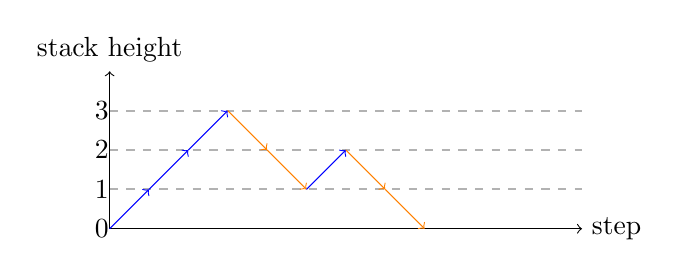
\begin{tikzpicture}
    \draw[thick, dashed, opacity=0.3] (0,0.5) -- (6,0.5);
     \draw[thick, dashed, opacity=0.3] (0,1) -- (6,1);
      \draw[thick, dashed, opacity=0.3] (0,1.5) -- (6,1.5);
      \draw[->] (0,0) -- (6,0) node[right] {step};
      \draw[->] (0,0) -- (0,2) node[above] {stack height};
     \draw[->, blue] (0,0) -- (0.5,0.5);
      \draw[->, blue] (0.5,0.5) -- (1,1);
      \draw[->, blue] (1,1) -- (1.5,1.5);
       \draw[->, orange] (1.5,1.5) -- (2,1);
    \draw[->, orange] (2,1) -- (2.5,0.5);
    \draw[->, blue] (2.5,0.5) -- (3,1);
    \draw[->, orange] (3,1) -- (3.5,0.5);
 \draw[->, orange] (3.5,0.5) -- (4,0);
\node (null) at (-0.1, 0) {0}; 
\node (one) at (-0.1, 0.5) {1}; 
\node (two) at (-0.1, 1) {2}; 
\node (three) at (-0.1, 1.5) {3}; 
    \end{tikzpicture}
\caption{Stack heights during the run of PDA.}
\label{oscb}
\end{figure}


PDA run $r$ is \textit{k-oscillating} if the harmonic of order $k$ is the greatest harmonic that occurs in $r$ after removing $0$ or more matching pairs. \textit{Bounded-oscillation languages} are languages accepted by pushdown automata with all runs $k$-oscillating. It is important that the problem whether a given CFL is a bounded-oscillation language is undecidable \cite{BoundOsc}.
\begin{example}
Consider Figure \ref{oscb}. It shows how the stack height changes during the run of a PDA. Corresponding well-nested word $\alpha(r)$ is $\bar{a}\bar{a}\bar{a}aa\bar{a}aa$. The greatest harmonic in this word is order 1 harmonic (moves forming harmonic are marked in bold, removed matching pairs are $(1, 8)$ and $(2, 5)$): $\bar{a}\bar{a}\mathbf{\bar{a}a}a\mathbf{\bar{a}a}a$, therefore oscillation of the run $r$ is 1.
\end{example}


The oscillation of a parse tree of a context-free grammar can be defined similiarly to the oscillation of a PDA run. Given a parse tree $t$, we define corresponding well-nested word $\alpha(t)$ inductively as follows:
\begin{itemize}
\item if $n$ is the root of $t$ then $\alpha(t) = \bar{a}\alpha(n)$
\item if $n$ is a leaf then $\alpha(n)=a$
\item if $n$ has $k$ children then $\alpha(n) = a\underbrace{\bar{a}...\bar{a}}_\text{$k$ times}\alpha(n_1)...\alpha(n_k)$
\end{itemize}


Moreover, given a PDA run $r$, there exists a corresponding parse tree $t$ with the same well-nested word $\alpha(t)=\alpha(r)$ and vice versa \cite{BoundOsc}.


The oscillation of a parse tree is closely related with its $dimension$. For each node $v$ in a tree $t$, its dimension $dim(v)$ is inductively defined as follows:
\begin{itemize}
\item if $v$ is a leaf, then $dim(v)$ = 0
\item if $v$ is an internal node with $k$ children $v_1, v_2, ..., v_k$ for $k \ge 1$, then 
$$
dim(v) = 
 \begin{cases}
   \max_{i \in \{1...k\}}dim(v_i) &\text{if there is a unique maximum}\\
   \max_{i \in \{1...k\}}dim(v_i)+1 &\text{otherwise}
 \end{cases}
$$
\end{itemize}


Dimension of a parse tree $t$ $dim(t)$ is a dimension of its root.  It is observable from the definition that dimension of a tree $t$ is the height of the largest perfect binary tree, which can be obtained from $t$ by contracting edges and accordingly identifying vertices. A tree with dimension $dim(t) = 2$ is illustrated in Figure \ref{oscbtree}.
\begin{figure}
\centering
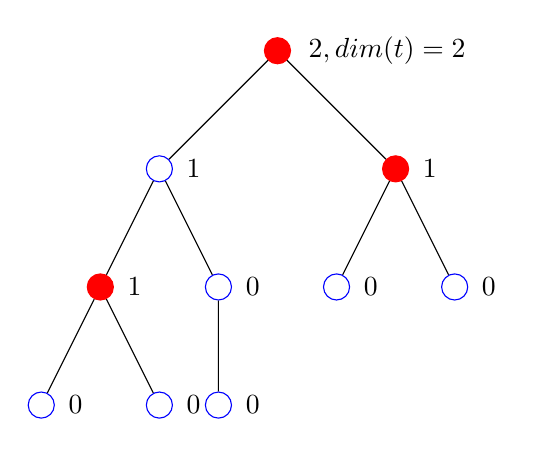
\begin{tikzpicture}[
level 1/.style={sibling distance=3cm},
level 2/.style={sibling distance=1.5cm}]
%\tikzstyle{every node}=[circle,draw]

\node[circle,draw] (Root) [ fill=red, red] {}
    child {
    node[circle,draw, blue] (l) {} 
    child { node[circle,draw, fill=red, red](ll) {}
            child { node[circle,draw, blue] (p) {} }
            child { node[circle,draw, blue] (pl) {} }
             }
    child { node[circle,draw, blue](lr) {} 
          child { node[circle,draw, blue] (plr) {} }
      }
}
child {
    node[circle,draw,  fill=red, red] (r) {}
    child { node[circle,draw, blue] (rl) {}} 
    child { node[circle,draw, blue] (rr) {} }
};
\node  [right=0.05cm of p] {0};
\node  [right=0.1cm of Root] {$2, dim(t)=2$};
\node  [right=0.05cm of l] {1};
\node  [right=0.05cm of r] {1};
\node  [right=0.05cm of ll] {1};
\node  [right=0.05cm of lr] {0};
\node  [right=0.05cm of pl] {0};
\node  [right=0.05cm of plr] {0};
\node  [right=0.05cm of rl] {0};
\node  [right=0.05cm of rr] {0};
\end{tikzpicture}
\caption{A tree $t$ with $dim(t)=2$. Nodes having children without unique maximum are filled.}
\label{oscbtree}            
\end{figure}


It is known that the dimension of parse trees and its oscillation are in linear relationship.

\begin{lemma}[\cite{BoundOsc}]
\label{boscdim}
Let a grammar $G = (\Sigma, N, P, S)$ be in Chomsky normal form and let $t$ be a parse tree of $G$. Then $osc(t) - 1 \le dim(t) \le 2osc(t)$.
\end{lemma}
\paragraph{Context-free language reachability.} 
A \textit{directed labeled graph} is a triple $D = (Q, \Sigma, \delta)$, where $Q$ is a finite set of nodes, $\Sigma$ is a finite set of alphabet symbols,
and $\delta \subseteq Q \times \Sigma \times Q$ is a finite set of labeled edges. Let $L(D)$ denote a graph language~--- a regular language, which is recognized by the NFA $(Q,\Sigma ,\delta ,Q, Q)$ obtained from $D$ by setting every state as inial and accepting.


Let $i\pi j$ denote a unique path between nodes $i$ and $j$ of the input graph and $l(\pi)$ denote a unique string obtained by concatenating edge labels along the path $\pi$. Then the CFL-reachability can be defined as follows.
\begin{definition}[Context-free language reachability]
Let $L \subseteq \Sigma^*$ be a context-free language and $D = (Q, \Sigma, \delta)$ be a directed labeled graph. Given two nodes $i$ and $j$ we say that $j$ is \textit{reachable} from $i$ if there exists a path $i \pi j$, such that $l(\pi) \in L$. 
\end{definition}
There are four varieties of CFL-reachability problems: all-pairs problem, single-source problem, single-target problem and single-source/single-target problem \cite{RepsBasic}. In this paper we consider all-pairs problem. The \textit{all-pairs problem} is to determine all pairs of nodes $i$ and $j$ such that $j$ is reachable from $i$. 




\section{Matrix-based CFPQ algorithm for all-path query semantics}
\label{sec:all-path-algo}
In this section, we introduce the AllPathIndex structure which is used as a base of our solution for all-path query semantics. Also, we propose the matrix-based algorithm for CFPQ w.r.t. the all-path query semantics.

\subsection{AllPathIndex}
Our algorithm is based on Azimov's CFPQ algorithm~\cite{Azimov:2018:CPQ:3210259.3210264} which is based on matrix operations.
This algorithm reduces CFPQ to operations over Boolean matrices and as a result, allows one to use high-performance linear algebra libraries and utilize modern parallel hardware for CFPQ.

Note, that the algorithm computes not only the context-free relation $R_{G,D}$ but also a set of context-free relations $R_{G_A,D} \subseteq V \times V$ for every $A \in N$ where $G_A = (N, \Sigma, P, A)$.
Thus it provides information about paths that form words derivable from any nonterminal $A \in N$.

We use an idea similar to one that was used for the CFPQ with single-path query semantics in~\cite{10.1145/3398682.3399163}. We store additional information in matrices to be able to restore all paths which form words derivable from any nonterminal in the given grammar.

In order to do this, we introduce the 
$$\textit{AllPathIndex} = (\textit{left},\textit{right},\textit{middles})$$ 
--- the elements of matrices that describe the found paths as concatenations of two smaller paths and help to restore each path after the index creation. Here \textit{left} and \textit{right} stand for the indexes of starting and ending vertices in the founded path, \textit{middles} --- the set of indexes of intermediate vertices used in the concatenation of two smaller paths. When we do not find the path for some vertex pair $i,j$, we use the $\textit{AllPathIndex} = \bot = (0,0,\emptyset)$.

Additionally, we will use the notation of \textit{proper matrix} which means that for every element of the matrix with indexes $i,j$ it either $\textit{AllPathIndex} = (i,j,\_)$ or $\bot$.

For proper matrices we use a binary operation $\otimes$ defined for AllPathIndexes \mbox{$AP_1, AP_2$} which are not equal to $\bot$ and with $AP_1.\textit{right} = AP_2.\textit{left}$ as
\begin{align*}
	AP_1 \otimes AP_2 = (&AP_1.left, AP_2.right, \{AP_1.right\}).
\end{align*}

And if at least one operand is equal to $\bot$ then $AP_1 \otimes AP_2 = \bot$.

For proper matrices we also use a binary operation $\oplus$ defined for AllPathIndexes \mbox{$AP_1, AP_2$} which are not equal to $\bot$ with $AP_1.\textit{left} = AP_2.\textit{left}$ and $AP_1.\textit{right} = AP_2.\textit{right}$ as
\begin{align*}
	AP_1 \otimes AP_2 = (&AP_1.left, AP_1.right, AP_1.middles \cup AP_2.middles).
\end{align*}
If only one operand is equal to $\bot$ then $AP_1 \oplus AP_2$ equal to another operand. If both operands are equal to $\bot$ then $AP_1 \oplus AP_2 = \bot$.

Using $\otimes$ as multiplication of AllPathIndexes, and $\oplus$ as an addition, we can define a \emph{matrix multiplication}, \mbox{$a \odot b = c$}, where $a$ and $b$ are matrices of a suitable size, that have AllPathIndexes as elements, as $c_{i,j} = \bigoplus^{n}_{k=1}{a_{i,k} \otimes b_{k,j}}.$

Also, we use the element-wise $+$ operation on matrices $a$ and $b$ with the same size: \mbox{$a + b = c$}, where $c_{i,j} = a_{i,j} \oplus b_{i,j}.$


\subsection{The matrix-based algorithm}
We introduce the matrix-based algorithm for CFPQ w.r.t. the all-path query semantics (see Listing~\ref{lst:algo1}). This algorithm is a modification of Azimov's matrix-based algorithm for CFPQ and it constructs the set of matrices $T$ with AllPathIndexes as elements.
Let $G = (N, \Sigma, P, S)$ be the input context-free grammar, $D = (V, E, \Sigma)$ be the input graph.
The result of the algorithm is a set of matrices $T$ which stores information about all paths in the graph $D$ that form a word derivable from some nonterminal of the context-free grammar $G$. Note that in line 4 we add the special value $n$ to the $T^{A_i}_{k,l}.middles$ to specify that this path is a single-edge path or an empty path $\pi_{\varepsilon}$.

\begin{algorithm}
\small
\begin{algorithmic}[1]
\floatname{algorithm}{Listing}
\caption{CFPQ algorithm for all-path query semantics}
\label{lst:algo1}
\Function{AllPathCFPQ}{\par
\hskip\algorithmicindent $D = (V, E, \Sigma)$, \par
\hskip\algorithmicindent $G=(N,\Sigma,P,S)$} \Comment{Grammar in WCNF}\par
\State{$n \gets$ |V|}
\State{$T \gets \{T^{A} \mid A \in N, T^{A}$ is a matrix $n \times n$, $T^{A}_{i,j} \gets \bot$ \} }
\ForAll{$(i,x,j) \in E$, $A \mid A \to x \in P$}
%\Comment{Matrices initialization}
%\For{$A_k \mid A_k \to x \in P$}
{$T^{A}_{i,j} \gets (i,j,\{n\})$}
%\EndFor
\EndFor
\ForAll{$A \mid A \to \varepsilon \in P$}
{$T^{A}_{i,i} \gets (i,i,\{n\})$}
\EndFor

\While{any matrix in $T$ is changing}
%\Comment{Transitive closure calculation}
\ForAll{$A \to B C \in P$ where $T^{B}$ or $T^{C}$ are changed}
\State{ $T^{A} \gets T^{A} + (T^{B} \odot T^{C})$ } 
\EndFor
\EndWhile
\State \Return $T$
\EndFunction

\end{algorithmic}
\end{algorithm}

After constructing a set of matrices $T$ or so-called \textit{index}, we can construct a set of all paths $\pi$ between specified vertex pair $(i, j)$ and a non-terminal $A$ such that $A \xLongrightarrow[G]{*} l(\pi)$. The index $T$ already stores data about all paths derivable from each nonterminal. However, the
set of such paths can be infinite. From a practical perspective, it is necessary
to use lazy evaluation or limit the resulting set of paths in some other way.
For example, one can try to query some fixed number of paths or query paths
of fixed maximum length.

We propose the algorithm (see Listing~\ref{lst:algo2}) for extracting these paths. Our algorithm returns a set with the empty path $\pi_{\varepsilon}$ only if $i = j$ and $A \to \varepsilon \in P$. If the AllPathIndex for the given $i,j,A$ is equal to $\bot$ then our algorithm returns the empty set since such paths do not exist. Note that in line 19 we use
the operation $\cdot$ which naturally generalizes the path concatenation operation
by constructing all possible concatenations of path pairs from the given two
sets. It is assumed that the sets are computed lazily, to ensure the termination in case of an infinite number of paths.

\begin{algorithm}
	\small
	\begin{algorithmic}[1]
		\floatname{algorithm}{Listing}
		\caption{All paths extraction algorithm}
		\label{lst:algo2}		
		\Function{extractAllPaths}{$i, j, A, T=\{T^{A_i}\}, G=(N,\Sigma,P,S)$}
		\State{$index \gets T^{A}_{i,j}$ }
		
		\If{$index = \bot$}
		\State \Return $\emptyset$
		\Comment{Such paths do not exist}
		\EndIf
		
		\State{$n \gets $ size of the square matrix $T^{A}$}
		\State{$resultPaths \gets \emptyset$}
		
		\ForAll{$middle \in index.middles$}		
		\If{$middle = n$}  \Comment{Add single-edge or empty paths}
		\ForAll{$x \mid A \to x \in P$}
		\If{$(i,x,j) \in E$}
		\State{$resultPaths \gets resultPaths \cup \{((i,x,j))\}$}
		\EndIf
		\EndFor
		\If{$(i = j) \wedge (A \to \varepsilon \in P)$}
		\State{$resultPaths \gets resultPaths \cup \{\pi_{\varepsilon}\}$}
		\EndIf
		\Else \Comment{Add to result the concatenated paths from $i$ to $middle$ and from $middle$ to $j$}
		\ForAll{$A \to B C \in P$}
		\State{$index_B \gets T^{B}_{i,middle}$ }
		\State{$index_C \gets T^{C}_{middle,j}$ }
		\If{$(index_B \neq \bot) \wedge (index_C \neq \bot)$}
		\State{$lPaths \gets$ \Call{extractAllPaths}{$i, middle, B, T, G$}}
		\State{$rPaths \gets$ \Call{extractAllPaths}{$middle, j, C, T, G$}}
		\State{$resultPaths \gets resultPaths \cup lPaths \cdot rPaths$}
		\EndIf
		\EndFor
		\EndIf
		\EndFor
		\State \Return $resultPaths$
		\EndFunction
	\end{algorithmic}
\end{algorithm}

\subsection{Correctness}

The following correctness theorem holds.

\begin{mytheorem}\label{thm:correct}
Let $G = (N, \Sigma, P, S)$ be the input context-free grammar, $D = (V, E, \Sigma)$ be the input graph, and $T$ be a set of matrices returned by the algorithm in Listing~\ref{lst:algo1}. Then for any $i, j$ and for any non-terminal $A \in N$, $index = T^A_{i,j}$ and $index = (i,j,middles) \neq \bot$ iff $(i,j) \in R_{G_A, D}$ and there is a path $\pi$ from vertex $i$ to $j$ such that $l(\pi) \in G_A = (N,\Sigma,P,A)$.
\end{mytheorem}
\begin{proof}[Proof sketch]
	At each iteration of the main cycle in lines 6-8 of the algorithm, the new paths corresponding to nonterminals $A \in N$ are considered using the rules $A \to B C \in P$. These new paths are obtained by the concatenation of two smaller paths corresponding to the nonterminals $B$ and $C$. At the initialization step of the algorithm in lines 3-5, we consider all single-edge or empty paths corresponding to the derivation tree of height 1. Thus, it can be shown that at iteration $l$ of the main cycle we consider all paths $\pi$ such that there is a derivation tree of the height $h \leq l + 1$ for the string $l(\pi)$ and a context-free grammar $G_A$. Therefore, the theorem can be proved using the induction on the height of such derivation trees.	
\end{proof}

Now, using the theorem~\ref{thm:correct} and induction on the length of the path, it can be easily shown that the following theorem holds.

\begin{mytheorem}\label{thm:correct_extraction}
Let $G = (N, \Sigma, P, S)$ be the input context-free grammar, $D = (V, E, \Sigma)$ be the input graph, and $T$ be a set of matrices returned by the algorithm in Listing~\ref{lst:algo1}. Then for any $i, j$ and for any non-terminal $A \in N$ such that $index = T^A_{i,j}$ and $index = (i,j,middles) \neq \bot$, the algorithm in Listing~\ref{lst:algo2} for these parameters will return a set of all paths $\pi$ from vertex $i$ to $j$ such that $l(\pi) \in G_A = (N,\Sigma,P,A)$.
\end{mytheorem}

We can, therefore, determine whether $(i,j) \in R_{G, D}$ by asking whether $T^S_{i,j} = \bot$. Also, we can extract all paths which form a word from the context-free language $L(G)$ by using our algorithm in Listing~\ref{lst:algo2}. Thus, we show how the context-free path query evaluation w.r.t. the all-path query semantics can be solved in terms of matrix operations.

%\subsection{Complexity}

%Denote the number of elementary operations executed by the algorithm of multiplying two $n \times n$ matrices with PathIndexes as $MM(n)$. Also, denote the number of elementary operations, executed by the matrix element-wise + operation of two $n \times n$ matrices with PathIndexes as $MA(n)$. Since the line \textbf{7} of the algorithm in listing~\ref{lst:algo2} is executed no more than $|V|^2|N|$ times (for the same reasons as in the original paper~\cite{Azimov:2018:CPQ:3210259.3210264} of the matrix-based CFPQ algorithm), the following theorem holds.

%\begin{myproposition}\label{thm:time}
%	Let $D = (V,E)$ be a graph and let $G =(N,\Sigma,P)$ be a grammar. The algorithm in listing~\ref{lst:algo2} calculates the set of matrices $T$ in $O(|V|^2|N|^3(MM(|V|) + MA(|V|)))$.
%\end{myproposition}

%Also, denote the time complexity of the access to the PathIndex in the $n \times n$ matrix as $Access(n)$. Then the following theorem on the time complexity of the path extraction algorithm holds.

%\begin{myproposition}\label{thm:time_extraction}
%	Let $D = (V,E)$ be a graph, let $G =(N,\Sigma,P)$ be a grammar and $T$ be a set of matrices returned by the algorithm in listing~\ref{lst:algo2}. Then for any $i, j$ and for any non-terminal $A \in N$ such that $index = T^A_{i,j}$ and $index = (i,j,k,h,l) \neq \bot$, the algorithm in listing~\ref{lst:algo3} for these parameters calculates a path $i \pi j$ in $O(l \times N \times Access(|V|))$.
%\end{myproposition}

\subsection{An Example}
In this section, we provide a step-by-step demonstration of the proposed algorithms. %For this, we consider the example with the worst-case time complexity.

We run the query on a graph $D_1$, presented in Figure~\ref{fig:example_input_graph}. We provide a step-by-step demonstration of the work of algorithm in Listing~\ref{lst:algo1} with the given graph $D$ and grammar $G_1^{\text{wcnf}}$ from section~\ref{sec:preliminaries}. After the matrix initialization in lines \textbf{3-5} of this algorithm, we have a set of matrices $T^{(1)}$, presented in Figure~\ref{ExampleQueryInitMatrix}.

{\footnotesize
	\begin{figure}[h]
		\[
		T^{(1),A} = \begin{pmatrix}
			\bot & (0,1,\{4\})       & \bot & \bot       \\
			\bot & \bot & (1,2,\{4\})       & \bot \\
			(2,0,\{4\})       & \bot & \bot & \bot \\
			\bot       & \bot & \bot & \bot \\
		\end{pmatrix}
		\]
		\[
		T^{(1),B} = \begin{pmatrix}
			\bot & \bot       & \bot & (0,3,\{4\})       \\
			\bot & \bot & \bot       & \bot \\
			\bot       & \bot & \bot & \bot \\
			(3,0,\{4\})      & \bot & \bot & \bot \\
		\end{pmatrix}
		\]
		\caption{The initial matrices for the example query. The PathIndexes $T^{(1),S_1}_{i,j}$ and $T^{(1),S}_{i,j}$ are equal to $\bot$ for every $i,j$}
		\label{ExampleQueryInitMatrix}
	\end{figure}
}

After the initialization, the only matrices which will be updated are $T^{S_1}$ and $T^{S}$. These matrices obtained after the first loop iteration is shown in Figure~\ref{ExampleQueryFirstIteration}.

{\footnotesize
	\begin{figure}[h]
		\[
		T^{(2),S} = \begin{pmatrix}
			\bot & \bot       & \bot & \bot       \\
			\bot & \bot & \bot       & \bot \\
			\bot       & \bot & \bot & (2,3,\{0\}) \\
			\bot       & \bot & \bot & \bot \\
		\end{pmatrix}
		\]
		\caption{The first iteration of computing the transitive closure for the example query. The PathIndexes $T^{(1),S_1}_{i,j}$ are equal to $\bot$ for every $i,j$}
		\label{ExampleQueryFirstIteration}
	\end{figure}
}

When the algorithm at some iteration finds new paths for some non-terminal in the graph $D_1$, then it adds corresponding AllPathIndexes to the matrix for this non-terminal. For example, after the first loop iteration, AllPathIndex $(2,3,\{0\})$ is added to the matrix $T^{S}$. This AllPathIndex is added to the element with a row index $i = 2$ and a column index $j = 3$. This means, that there is a path $\pi$ from the vertex 2 to the vertex 3, such that $S \xLongrightarrow[G_1^{\text{wcnf}}]{*} l(\pi)$ and this path obtained by concatenation of two smaller paths via vertex 0.

The calculation of the index $T$ is completed after $k$ iterations, when a fixpoint is reached: $T^{(k)} = T^{(k-1)}$. For the example query, $k = 14$ since $T_{14} = T_{13}$. The resulted matrix for non-terminal $S$ is presented in Figure~\ref{ExampleQueryFinalMatrices}.

{\footnotesize
	\begin{figure}[h]
		\[
		T^{(14),S} = \begin{pmatrix}
			(0,0,\{1\}) & \bot       & \bot & (0,3,\{1\})       \\
			(1,0,\{2\}) & \bot & \bot       & (1,3,\{2\}) \\
			(2,0,\{0\})       & \bot & \bot & (2,3,\{0\}) \\
			\bot       & \bot & \bot & \bot \\
		\end{pmatrix}
		\]
		\caption{The final matrix for non-terminal $S$ after computing the index}
		\label{ExampleQueryFinalMatrices}
	\end{figure}
}

Now, after constructing the index, we can construct the context-free relation $$R_{G_1^{\text{wcnf}}, D_1}=\{(0,0),(0,3),(1,0),(1,3),(2,0),(2,3)\}.$$

In the relation $R_{G_1^{\text{wcnf}}, D_1}$, we have all vertex pairs corresponding to paths, whose labeling is in the language $L(G_1^{\text{wcnf}}) = \{a^n b^n \mid n \geq 1\}$. Using the algorithm in Listing~\ref{lst:algo2} we can restore paths for each vertex pair from the context-free relation. For example, given $i=j=0$, non-terminal $S$, set of resulted matrices $T$, and context-free grammar $G_1^{\text{wcnf}}$, the algorithm in Listing~\ref{lst:algo2} returns an infinite set of all paths from vertex 0 to vertex 0 whose labeling form words from the following set $\{a^6 b^6, a^{12} b^{12}, a^{18} b^{18}, \ldots \}$. Following the path corresponding to the word $a^{6m} b^{6m}$, we will go through the cycle with $a$ labels $2m$ times and through the cycle with $b$ labels $3m$ times for all $m \geq 1$.
\section{Evaluation}

The goal of this evaluation is to investigate the applicability of the proposed algorithm to both regular and context-free path querying.
We measured the execution time of the index creation which solves the reachability problem for both kinds of queries.
The execution time for CFPQ was compared with the Azimov's algorithm for CFPQ reachability.
We also investigated the practical applicability of paths extraction algorithm to both regular and context-free path queries.

For evaluation, we used a PC with Ubuntu 18.04 installed.
It has Intel core i7-6700 CPU, 3.4GHz, and DDR4 64Gb RAM.
We only measure the execution time of the algorithms themselves, thus we assume an input graph is loaded into RAM in the form of its adjacency matrix in the sparse format.
Note, that the time needed to load an input graph into the RAM is excluded from the time measurements.

\subsection{RPQ Evaluation}

To investigate the applicability of the proposed algorithm for regular path querying we gathered a dataset which consists of both real-world and synthetically generated graphs.
We generated the queries from the most popular RPQ templates.

\subsubsection{Dataset}

We gathered several graphs which represent real-world data from different areas and are frequently used for evaluation of the graph querying algorithms.
Namely, the dataset consists of three parts.
The first part is the set of LUBM graphs\footnote{Lehigh University Benchmark (LUBM) web page: \url{http://swat.cse.lehigh.edu/projects/lubm/}. Access date: 07.07.2020.}~\citep{10.1016/j.websem.2005.06.005} which have different numbers of vertices.
The second one is the set of graphs from Uniprot database\footnote{Universal Protein Resource (UniProt) web page: \url{https://www.uniprot.org/}. All files used can be downloaded via the link: \url{ftp://ftp.uniprot.org/pub/databases/uniprot/current_release/rdf/}. Access date: 07.07.2020.}: \textit{proteomes}, \textit{taxonomy} and \textit{uniprotkb}.
The~last part consists of the RDF files \textit{mappingbased\_properties} from DBpedia\footnote{DBpedia project web site: \url{https://wiki.dbpedia.org/}. Access date: 07.07.2020.} and \textit{geospecies}\footnote{The Geospecies RDF: \url{https://old.datahub.io/dataset/geospecies}. Access date: 07.07.2020.}.
A brief description of the graphs in the dataset is presented in Table~\ref{tbl:graphs_for_rpq}.

\begin{table}
    \centering
\caption{Graphs for RPQ evaluation}
\label{tbl:graphs_for_rpq}
{

\rowcolors{2}{black!2}{black!10}
\begin{tabular}{|l|c|c|}
\hline
Graph & \#V & \#E  \\
\hline
\hline
LUBM1k  & 120 926 & 484 646 \\
LUBM3.5k  & 358 434 & 144 9711 \\
LUBM5.9k  & 596 760 & 2 416 513 \\
LUBM1M   & 1 188 340 & 4 820 728 \\
LUBM1.7M & 1 780 956 & 7 228 358 \\
LUBM2.3M & 2 308 385 & 9 369 511 \\
\hline
Uniprotkb & 6 442 630 & 24 465 430 \\
Proteomes & 4 834 262 & 12 366 973 \\
Taxonomy & 5 728 398 & 14 922 125 \\
\hline
Geospecies & 450 609 & 2 201 532 \\
Mappingbased\_properties & 8 332 233 & 25 346 359 \\
\hline
\end{tabular}
}
\end{table}


Queries for evaluation were generated from the templates for the most popular RPQs, specifically the queries presented in Table 2 in~\cite{Pacaci2020RegularPQ} and in Table 5 in~\cite{Wang2019}.
These query templates are presented in Table~\ref{tbl:queries_templates}.
We generate 10 queries for each template and each graph.
The most frequent relations from the given graph were used as symbols in the query template\footnote{Used generator is available as part of CFPQ\_data project: \url{https://github.com/JetBrains-Research/CFPQ_Data/blob/master/tools/gen_RPQ/gen.py}. Access data: 07.07.2020.}.
We used the same set of queries for all LUBM graphs to investigate scalability of the proposed algorithm.

\begin{table}
    \centering
\caption{Queries templates for RPQ evaluation}
\label{tbl:queries_templates}
{\small
\renewcommand{\arraystretch}{1.2}
\rowcolors{2}{black!2}{black!10}
\begin{tabular}{|c|c||c|c|}
\hline

Name & Query & Name & Query \\
\hline
\hline
$Q_1$   & $a^*$                               & $Q_9^5$    & $(a \mid b \mid c \mid d \mid e)^+$                     \\
$Q_2$   & $a\cdot b^*$                        & $Q_{10}^2$ & $(a \mid b) \cdot c^*$                                  \\
$Q_3$   & $a \cdot b^* \cdot c^*$             & $Q_{10}^3$ & $(a \mid b \mid c)  \cdot d^*$                          \\
$Q_4^2$ & $(a \mid b)^*$                      & $Q_{10}^4$ & $(a \mid b \mid c \mid d)  \cdot e^*$                   \\
$Q_4^3$ & $(a \mid b \mid c)^*$               & $Q_{10}^5$ & $(a \mid b \mid c \mid d \mid e)  \cdot f^*$            \\
$Q_4^4$ & $(a \mid b \mid c \mid d)^*$        & $Q_{10}^2$ & $a \cdot b$                                             \\
$Q_4^5$ & $(a \mid b \mid c \mid d \mid e)^*$ & $Q_{11}^3$ & $a \cdot b \cdot c$                                     \\
$Q_5$   & $a \cdot b^* \cdot c$               & $Q_{11}^4$ & $a \cdot b \cdot c \cdot d$                             \\
$Q_6$   & $a^* \cdot b^*$                     & $Q_{11}^5$ & $a \cdot b \cdot c \cdot d \cdot f$                     \\
$Q_7$   & $a \cdot b \cdot c^*$               & $Q_{12}$   & $(a \cdot b)^+ \mid  (c \cdot d)^+$                     \\
$Q_8$   & $a? \cdot b^*$                      & $Q_{13}$   & $(a \cdot(b \cdot c)^*)^+ \mid  (d \cdot f)^+$          \\
$Q_9^2$ & $(a \mid b)^+$                      & $Q_{14}$   & $(a \cdot b \cdot (c \cdot d)^*)^+  \cdot (e \mid f)^*$ \\
$Q_9^3$ & $(a \mid b \mid c)^+$               & $Q_{15}$   & $(a \mid b)^+ \cdot (c \mid d)^+$                       \\
$Q_9^4$ & $(a \mid b \mid c \mid d)^+$        & $Q_{16}$   & $a \cdot b \cdot (c \mid d \mid e)$                     \\
\hline
\end{tabular}
}
\end{table}


\subsubsection{Results}

We averaged the execution time of index creation over 5 runs for each query.
Index creation time for LUBM graphs set is presented in Figure~\ref{fig:lubm_all_qs}.
We can see that evaluation time depends on the query: there are queries which evaluate in less than 1 second even for the largest graphs ($Q_2$, $Q_5$, $Q_{11}^2$, $Q_{11}^3$), while the worst time is 6.26 seconds ($Q_{14}$).
The execution time of our algorithm is comparable with the recent results for the same graphs and queries implemented on a distributed system over 10 nodes~\citep{Wang2019}, while we use only one node.
We conclude that our algorithm demonstrates reasonable performance to be applied to the real-world data analysis.
%\cho{Note that the accurate comparison of different approaches may be a promising direction of future research.}

\begin{figure}
    \centering
   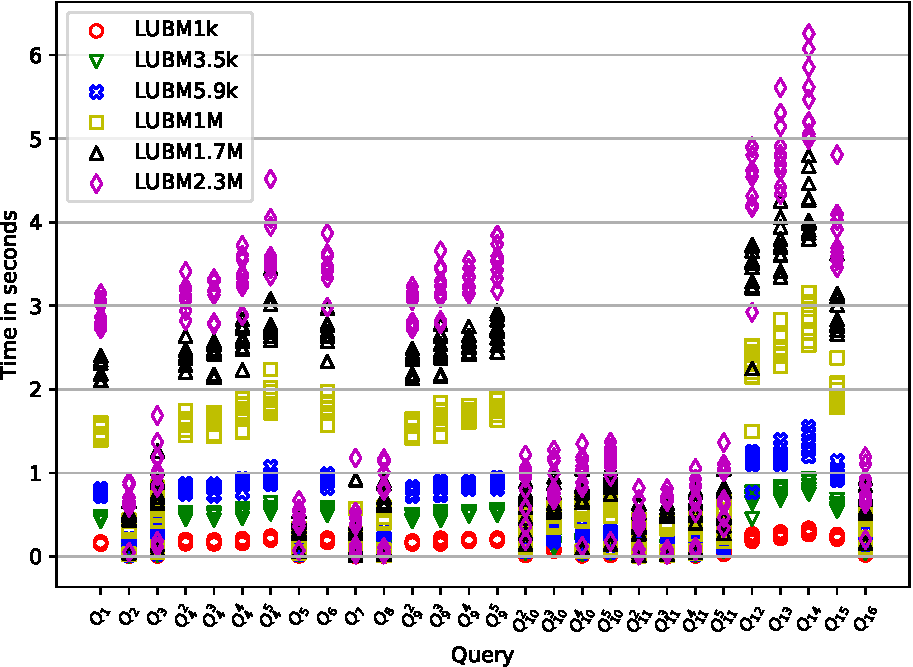
\includegraphics[width=0.6\textwidth]{data/LUBM_all.pdf}
   \caption{Index creation time for LUBM graphs}
   \label{fig:lubm_all_qs}
\end{figure}

Index creation time for each query on the real-world graphs is presented in Figure~\ref{fig:other_all_qs}.
We can see that querying small graphs requires more time than querying bigger graphs in some cases.
For example, conseder $Q_{10}^4$: querying the \textit{geospecies} graph (450k vertices) in some cases requires more time than querying of \textit{mappingbased\_properties} (8.3M vertices) and \textit{taxonomy} (5.7M vertices).
We conclude that the evaluation time depends on the inner structure of a graph.
On the other hand, \textit{taxonomy} querying in many cases requires significantly more time than for other graphs, while \textit{taxonomy} is not the biggest graph.
Finally, in most cases query execution lasts less than 10 seconds, even for bigger graphs, and no query requires more than 52.17 seconds.

\begin{figure}
    \centering
   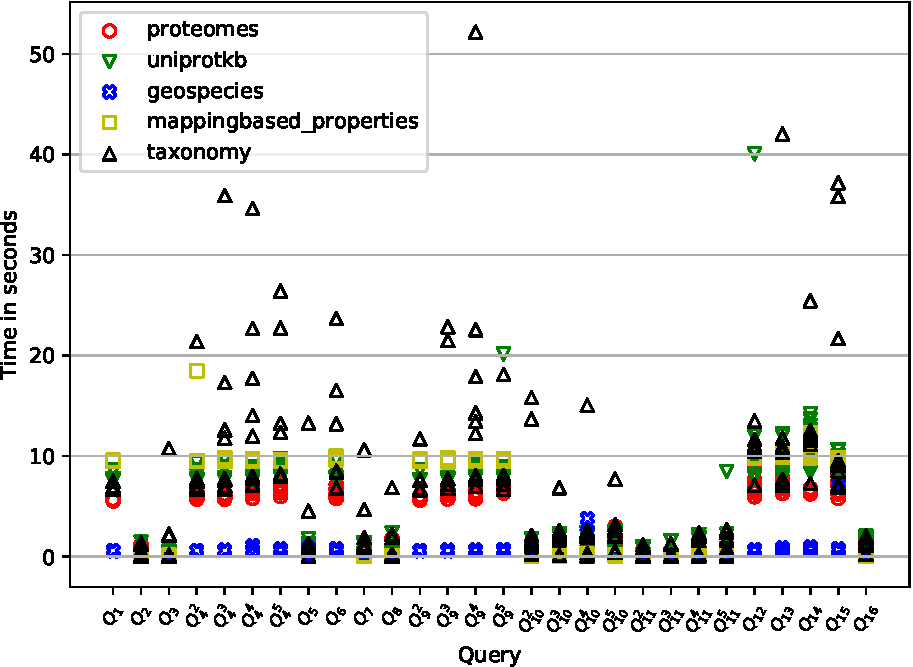
\includegraphics[width=0.6\textwidth]{data/other_all.pdf}
   \caption{Index creation time for real-world RDFs}
   \label{fig:other_all_qs}
\end{figure}

%We evaluate path extraction for queries which result in possibly long paths.
%Long paths usually require many iterations of transitive closure evaluation, thus we used the number of the iterations as a criterion to select the inputs for the evaluation.
%For each selected graph and query we measure paths extraction time for each reachable pair.
%Since the index can be reused from the previous step, we omit the time necessary to create the index.
%We limit by 10 the number of paths to extract.

%In Figures~\ref{fig:geo_tensors_rpq} and~\ref{fig:dbpedia_tensors_rpq} we show the time needed to extract a path of a specific length when only one path was extracted.
%The main observation is that time is linear on the path length, even if a generic path extraction procedure is used.

%\begin{figure}
%     \begin{subfigure}[b]{0.45\textwidth}
%         \centering
%         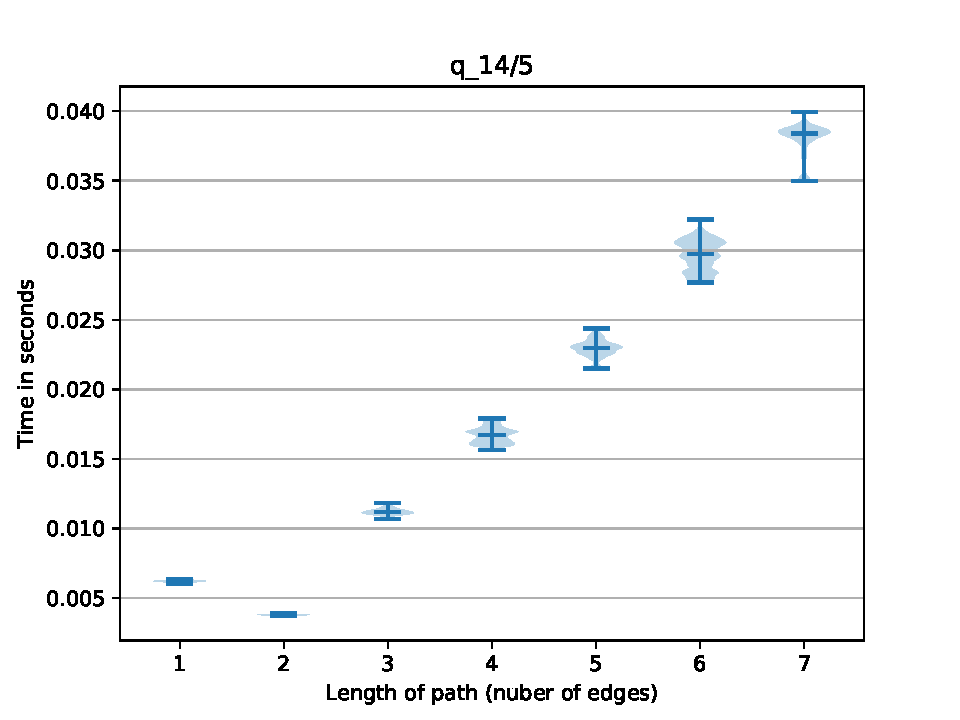
\includegraphics[width=\textwidth]{../paper/data/geo_rpq_single_path/q_14_5.pdf}
%         \caption{\footnotesize \textit{geospecies}, $Q_{14}$}
%         \label{fig:geo_tensors_rpq}
%     \end{subfigure}
%     ~\begin{subfigure}[b]{0.45\textwidth}
%         \centering
%         \includegraphics[width=\textwidth]{../paper/data/CF/Tensor_path/dbpedia_path_tensor.pdf}
%         \caption{\footnotesize \textit{mappingbased\_properties}, $Q_{4}^5$}
%         \label{fig:dbpedia_tensors_rpq}
%     \end{subfigure}\\
%     \begin{subfigure}[b]{0.45\textwidth}
%         \centering
%         \includegraphics[width=\textwidth]{../paper/data/CF/Matrix_CF/geo_path_matrix.pdf}
%         \caption{\footnotesize \textit{geospecies}, \textit{Geo}}
%         \label{fig:geo_matrix_cfpq}
%     \end{subfigure}
%     ~\begin{subfigure}[b]{0.45\textwidth}
%         \centering
%         \includegraphics[width=\textwidth]{../paper/data/CF/Tensor_path/geo_path_tensor.pdf}
%         \caption{\footnotesize \textit{geospecies}, \textit{Geo}}
%         \label{fig:geo_tensors_cfpq}
%     \end{subfigure}\\
%   \caption{Single path extraction for specific graph and query for our solution (\subref{fig:geo_tensors_rpq}, \%subref{fig:dbpedia_tensors_rpq}, \subref{fig:geo_tensors_cfpq}), and Azimov's (\subref{fig:geo_matrix_cfpq})}
%\end{figure}

\subsection{CFPQ Evaluation}

We evaluate the applicability of the proposed algorithm to CFPQ processing over real-world graphs on a number of classic cases and compare them with the Azimov's algorithm.
Currently only a single path version of Azimov's algorithm exists, and we use its implementation using PyGraphBLAS. Note that it is not trivial to compare our results with the state-of-the-art results provided by~\cite{10.1145/3398682.3399163} (Azimov's algorithm) because our algorithm computes significantly more information. While the state-of-the-art solution computes only reachability facts or a single-path semantics, our algorithm computes data necessary to restore all possible paths.

\subsubsection{Dataset}

We use CFPQ\_Data\footnote{CFPQ\_Data is a dataset for CFPQ evaluation which contains both synthetic and real-world data and queries \url{https://github.com/JetBrains-Research/CFPQ\_Data}. Access date: 07.07.2020.} dataset for evaluation.
Namely, we use relatively big RDF files and respective same-generation queries $G_1$~(Eq.~\ref{eqn:g_1}) and $G_2$~(Eq.~\ref{eqn:g_2}) which are used in other works for CFPQ evaluation.
We also use the $Geo$~(Eq.~\ref{eqn:geo}) query provided by~\cite{Kuijpers:2019:ESC:3335783.3335791} for \textit{geospecies} RDF.
Note that we use $\overline{x}$ notation in queries to denote the inverse of $x$ relation and the respective edge.
\begin{align}
\begin{split}
\label{eqn:g_1}
S \to & \overline{\textit{subClassOf}} \ \ S \ \textit{subClasOf} \mid \overline{\textit{type}} \ \ S \ \textit{type}\\   & \mid \overline{\textit{subClassOf}} \ \ \textit{subClasOf} \mid \overline{\textit{type}} \ \textit{type}
\end{split}
\end{align}
\begin{align}
\begin{split}
\label{eqn:g_2}
S \to \overline{\textit{subClassOf}} \ \ S \ \textit{subClasOf} \mid \textit{subClassOf}
\end{split}
\end{align}
\begin{align}
\begin{split}
\label{eqn:geo}
S \to & \textit{broaderTransitive} \ \  S \ \overline{\textit{broaderTransitive}} \\
      & \mid \textit{broaderTransitive} \ \  \overline{\textit{broaderTransitive}}
\end{split}
\end{align}
\begin{align}
\begin{split}
\label{eqn:ma}
S & \to \overline{d} \ V \ d \\
V & \to ((S?) \overline{a})^* (S?) (a (S?))^*
\end{split}
\end{align}

Additionally we evaluate our algorithm on memory aliases analysis problem: a well-known problem which can be reduced to CFPQ~\citep{Zheng:2008:DAA:1328897.1328464}.
To do it, we use some graphs built for different parts of Linux OS kernel (\textit{arch}, \textit{crypto}, \textit{drivers}, \textit{fs}) and the query $MA$~(Eq.~\ref{eqn:ma})~\citep{10.1145/3093336.3037744}.
The detailed data about all the graphs used is presented in Table~\ref{tbl:graphs_for_cfpq}.

{\setlength{\tabcolsep}{0.3em}
\begin{table}
    \centering
{
\caption{Graphs for CFPQ evaluation: \textit{bt} is broaderTransitive, \textit{sco} is subCalssOf}
\label{tbl:graphs_for_cfpq}
\scriptsize
\rowcolors{2}{black!2}{black!10}
\begin{tabular}{|l|c|c|c|c|c|c|c|}
\hline
Graph          & \#V       & \#E        & \#sco & \#type &\#bt & \#a  & \#d \\
\hline
\hline
eclass\_514en  & 239 111    & 523 727    & 90 512    & 72 517    &        ---        & ---  & --- \\
enzyme         & 48 815     & 109 695    & 8 163     & 14 989    &        ---        & ---  & --- \\
geospecies     & 450 609    & 2 201 532  & 0         & 89 062    &        20 867     & ---  & --- \\
go             & 272 770    & 534 311    & 90 512    & 58 483    &        ---        & ---  & --- \\
go-hierarchy   & 45 007     & 980 218    & 490 109   & 0         &        ---        & ---  & --- \\
taxonomy       & 5 728 398  & 14 922 125 & 2 112 637 & 2 508 635 &        ---        & ---  & --- \\
\hline
arch           & 3 448 422  & 5 940 484  &      ---     &  ---   &        ---        & 671 295 & 2 298 947 \\
crypto         & 3 464 970  & 5 976 774  &      ---     &  ---   &        ---        & 678 408 & 2 309 979 \\
drivers        & 4 273 803  & 7 415 538  &      ---     &  ---   &        ---        & 858 568 & 2 849 201 \\
fs             & 4 177 416  & 7 218 746  &      ---     &  ---   &        ---        & 824 430 & 2 784 943 \\
\hline
\end{tabular}
}
\end{table}
}
\subsubsection{Results}

We averaged the index creation time over 5 runs for both single-path Azimov's algorithm (\textbf{Mtx}) and the proposed algorithm (\textbf{Tns}) (see Table~\ref{tbl:CFPQ_index}).

{\setlength{\tabcolsep}{0.2em}
  \begin{table}
    \centering
    \caption{CFPQ evaluation results, time is measured in seconds}
    \label{tbl:CFPQ_index}
    \rowcolors{4}{black!2}{black!10}
    \small
    \begin{tabular}{| l | c | c | c | c | c | c | c | c |}
      \hline

      \multirow{2}{*}{Name}  & \multicolumn{2}{c|}{$G_1$} & \multicolumn{2}{c|}{$G_2$} & \multicolumn{2}{c|}{\textit{Geo}} & \multicolumn{2}{c|}{\textit{MA}}\\
      \cline{2-9}
                      & Tns    & Mtx    & Tns  & Mtx  & Tns   & Mtx   & Tns     & Mtx \\
      \hline
      \hline
      eclass\_514en   & 0.24   & 0.27   & 0.25 & 0.26 & ---   & ---   & ---     & ---\\
      enzyme          & 0.03   & 0.04   & 0.02 & 0.01 & ---   & ---   & ---     & ---\\
      geospecies      & 0.08   & 0.06   & $0^{*}$ & 0.01 & 26.12 & 16.58 & ---     & ---\\
      go-hierarchy    & 0.16   & 1.43   & 0.23 & 0.86 & ---   & ---   & ---     & ---\\
      go              & 1.56   & 1.74   & 1.21 & 1.14 & ---   & ---   & ---     & ---\\
      pathways        & 0.01   & 0.01   & 0.01 & 0.01 & ---   & ---   & ---     & ---\\
      taxonomy        & 4.81   & 2.71   & 3.75 & 1.56 & ---   & ---   & ---     & ---\\
      \hline
      arch            & ---    & ---    & ---  & ---  & ---   & ---   & 262.45  & 195.51  \\
      crypto          & ---    & ---    & ---  & ---  & ---   & ---   & 267.52  & 195.54  \\
      drivers         & ---    & ---    & ---  & ---  & ---   & ---   & 1309.57 & 1050.78 \\
      fs              & ---    & ---    & ---  & ---  & ---   & ---   & 470.49  & 370.73  \\
      \hline
    \end{tabular}
  \end{table}
}

Best to our knowledge, the proposed algorithm is the first algorithm that provides information about all paths of interest (Azimov's algorithm computes information about only one path).
The direct comparison with other solutions is impossible, and we just estimate the running time of our algorithm for a small number of cases.
Namely, we extract all paths with length not greater than 20 edges between all pairs of vertices from indeces created for graphs \textit{go} and \textit{eclass\_514en} and query $G_1$.
Paths extraction for one pair of vertices requires 2.64 seconds averaged over all pairs for \textit{go} graph. The~maximal time is 4699 seconds and 217737 paths were extracted during this time. The average number of paths between two vertices is 184.
For \textit{eclass\_514en} paths extraction for one pair of vertices requires 1.27 seconds averaged over all pairs. The~maximal time is 8.04 seconds and only one path is extracted during this time. The average number of paths between two vertices is 3.
We can see that paths can be extracted in a reasonable time, but a detailed analysis of paths extraction algorithm performance depends on graphs structure.

%Comparison of paths extraction is presented in Figures~\ref{fig:geo_matrix_cfpq} and~\ref{fig:geo_tensors_cfpq}.
%While both methods demonstrate linear time on the length of the extracted path, our generic solution is more than 1000 times slower than Azimov's single path extraction procedure.
%We conclude that current generic all-path extraction procedure is not optimal for single path extraction.

\subsection{Conclusion}

We conclude that the proposed algorithm is applicable to real-world data processing: the algorithm allows one to solve both the reachability problem and to extract paths of interest in a reasonable time even using naive implementation.
While index creation time (reachability query evaluation) is comparable with other existing solutions, paths extraction procedure should be improved in the future. However, the state-of-the-art solution computes only reachability facts or a single-path semantics, whereas our algorithm computes data necessary to restore all possible paths (all-paths semantics).
Finally, a detailed comparison of the proposed solution with other algorithms for CFPQ and RPQ is required.

To summarize the overall evaluation, the proposed algorithm is applicable to both RPQ and CFPQ over real-world graphs.
Thus, the proposed solution is a promising unified algorithm for both RPQ and CFPQ evaluation.

\section{Conclusion}

Conclusion, current state, results.

Future work. Library extension up to full GraphBLAS API implementation.

LaGraph on F\# .NET.

Evaluation. Comparison with other implementations on different devices.
Manual implementation versus translation.  

Another direction of future work is Brahma.FSharp improvements. 
First of all, it is necessary to support discriminated unions to make it possible to express custom semirings such as \texttt{Min-Plus}, as presented in listing~\ref{lst_example}. 

Also, it is necessary to add high-level abstractions for asynchronous programming, and for multi-GPU programming.
Such mechanisms can be naturally expressed in F\# with native primitives for asynchronous programming.

fusion and other optimizations.


\begin{acks}
	The research was supported by the Russian Science Foundation, grant \textnumero 18-11-00100.
\end{acks}

\balance

%%
%% The next two lines define the bibliography style to be used, and
%% the bibliography file.
\bibliographystyle{ACM-Reference-Format}
\bibliography{all-path-matrix-cfpq}

%%
%% If your work has an appendix, this is the place to put it.
%% Please note that all the content must fit within the page limits, including any appendices.
%\appendix
%
%\section{Research Methods}
% ...

\end{document}
\endinput




